

\lstdefinestyle{yaml}{
     basicstyle=\color{red}\footnotesize,
     rulecolor=\color{black},
     string=[s]{'}{'},
     stringstyle=\color{red},
     comment=[l]{:},
     commentstyle=\color{black},
     morecomment=[l]{-}
 }
\chapter{Docker} \label{ch:docker}


Negli ultimi anni numerose aziende che forniscono servizi agli utenti si sono trovate in serie difficoltà a causa dell' aumento sempre costante del numero
dei propri utenti e delle richieste di questi ultimi. Tali aziende si sono trovate quindi nella posizione di dover incrementare proporzionalmente le loro risorse disponibili, sia hardware che software, e di dover
assumere sempre più frequentemente del personale altamente specializzato per gestirle. Questa situazione di crisi ha portato ad un cambio di prospettiva in ambito aziendale, orientando l'attenzione verso un sistema di virtualizzazione
basato sull'utilizzo dei container invece che con le classiche macchine virtuali. Così facendo si è trovata una valida soluzione a questo problema, in quanto grazie alle loro caratteristiche i container consentono di garantire
la qualità del servizio offerto dalle aziende, ottimizzando l'utilizzo delle risorse hardware già in uso, senza la necessità di effettuare ulteriori investimenti significativi in hardware o personale aggiuntivo.\\
L'obiettivo di questo capitolo è di fornire una descrizione approfondita di una delle tecnologie più diffuse ed utilizzate in questo ambito, Docker\cite{docker-docs}. Inoltre viene anche descritto l'utilizzo di uno strumento, docker-compose, molto utile per 
creare e gestire applicazioni multi-container. Nella parte finale del capitolo è infine possibile trovare una descrizione e degli esempi su come eseguire il networking all'interno dei container.

\section{Differenze fra Container e Macchine Virtuali} 

Prima di scendere nello specifico descrivendo il funzionamento di docker all'interno di un sistema operativo è necessario definire nel dettaglio cosa sia una macchina virtuale e cosa un container e perchè è più efficiente la seconda soluzione rispetto alla prima.\\
Per quanto riguarda le macchine virtuali una definizione ci viene fornita dal sito ufficiale di VMware \cite{vmware}:\\
"Una Macchina Virtuale (VM) è una risorsa di elaborazione che utilizza software al posto di un computer fisico per eseguire programmi e distribuire applicazioni. Una o più macchine virtuali (guest) vengono eseguite su una macchina fisica (host). 
Ogni macchina virtuale esegue il proprio sistema operativo e funziona in modo separato dalle altre VM, anche quando sono tutte in esecuzione sulla stessa macchina host. Ciò significa che, ad esempio, una macchina virtuale con sistema operativo MacOS può essere eseguita su un PC fisico."\\

Sotto la prospettiva dei container, è possibile ottenere una definizione precisa consultando la documentazione ufficiale di Docker\cite{docker-container}.\\
"Un container è  un'unità standard di software che raggruppa il codice e tutte le sue dipendenze in modo che l'applicazione possa essere eseguita rapidamente e in modo affidabile da un ambiente di calcolo all'altro."\\

Seppur le due definizioni possano sembrare molto simili, la struttura software che sta dietro ad entrambe le tecniche di virtualizzazione è diversa, come viene mostrato nella seguente figura:\\


\begin{figure}[h]  % 'h' significa che la figura viene posizionata qui
    \centering
    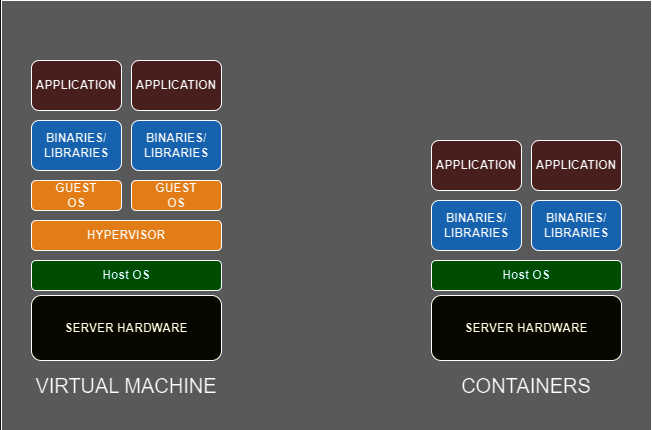
\includegraphics[width=1\textwidth]{VMvsContainers.png}  % Sostituisci 'nome_immagine' con il nome del tuo file immagine e l'estensione
    \caption{Architettura Virtual Machine e Containers}
    \label{fig:VMvsContainers}
\end{figure}
 
Le macchine virtuali hanno infatti una struttura più complessa rispetto ai container. È infatti presente un hypervisor\cite{hypervisor}, che è un software che permette di creare e gestire le macchine virtuali in maniera veloce, efficiente, flessibile e portabile.
Sopra all'hypervisor ogni macchina virtuale ha il suo proprio sistema operativo, costringendo l'host OS ad allocare numerose risorse per istanziare anche solo 1 macchina virtuale. Si può notare come questa soluzione sia difficlmente scalabile perchè
ciò porta il server hardware sul quale poggia tutto il sistema ad essere ulteriormente stressato con l'aggiunta di ogni macchina virtuale. Viceversa, i container richiedono solo le risorse minime necessaria a fare funzionare l'applicazione di turno, installando solo i file binari e le librerie necessarie.\\
Più in generale le caratteristiche vantaggiose dei container rispetto alle macchine virtuali sono riassunte dalle seguenti parole chiave:\\


\begin{itemize}
    \item \textbf{Modularità}: avere la possibilità di creare un container per ogni possibile task permette di suddividere i container in vari moduli, ognuno che svolge una sepcifica funzione del progetto di riferimento. Operando in tale direzione, è possibile sviluppare progetti con un approccio Bottom-Up
        , portando ad un ambiente di testing e validation più veloce ed immediato sui singoli moduli.
    \item \textbf{Isolamento}: ogni container che esegue una immagine viene visto come un ambiente isolato, indipendente dagli altri container in esecuzione. Questo approccio semplifica notevolmente l'individuazione di possibili bug ed errori nel progetto.
    \item \textbf{Peso in Memoria}: come analizzato nel lavoro di Martin Lindström\cite{performance-container}, differentemente dalle macchine virtuali, i container sono delle virtualizzazioni molto più leggere e che richiedono meno risorse alla macchina ospitante. Questo è derivato dal fatto che i container contengono solo lo stretto necessario all'applicazione per funzionare correttamente,
        mentre le VM hanno bisogno anche di istanziare un proprio sistema operativo, che richiede una discreta quantità di spazio.
    \item \textbf{Scalabilità}: Avendo un peso molto ridotto rispetto alle macchine virtuali, la necessità di aumentare le performance e le dimensioni di un progetto trova nei container un ottimo fattore di scalabilità. È  infatti possibile scalare i sistemi sia verticalmente, perchè all'aumentare delle risorse del sistema operativo ospitante corrisponde un aumento della velocità di reazione dei container
    che orizzontalmente, perchè aggiungere una feature corrisponde nell'aggiungere un container al sistema già funzionante. 
    \item \textbf{Condivisone Risorse}: Attraverso i file di configurazione dei container è possibile condividere file con il container, che nell'ambiente isolato verranno considerate come risorse dedicate, anche se in realtà sono condivise. Ciò estende questa funzionalità se si mettono in comune le stesse risorse per più container. In questo caso sulle risorse verrà messo un lock che bloccherà le risorse fino a che
        uno dei container non abbia finito di utilizzarle, rilasciandole.
    \item \textbf{Fast Boot}:Non dovendo dipendere da nessun sistema operativo, i container possono avviarsi ed essere operativi molto più velocemente rispetto alle macchine virtuali.
    \item \textbf{Operazioni su disco}: Avendo un collegamento diretto con il sistema operativo le operazioni su  disco (scrittura, lettura e cancellazione) sono più veloci, portando ad un aumento delle performance per processi parallelizzabili.
\end{itemize}

\newpage

\section{Docker e la sua architettura}

Tra le piattaforme software disponibili per istanziare e gestire containers per applicazioni Docker riveste il ruolo di software leader nel settore.
Nato nel 2013 e progettato da Solomon Hykes nell'azienda dotCloud, Docker è un progetto open source. La differenza fondamentale dagli altri software è che
basa la maggior parte delle operazioni eseguibili su un demone chiamato appunto Docker, che svolge le operazioni di istanziazione dei container e la loro gestione.
Al fine di garantire ciò, il demone richiede come file di input delle \textit{"Immagini"}. Come è descritto nella documentazione di Docker\cite{docker-container}: 
"Un'immagine di container Docker è un pacchetto leggero, autonomo ed eseguibile di software che include tutto il necessario per eseguire un'applicazione: codice, runtime, strumenti di sistema, librerie di sistema e impostazioni."\\

L'architettura di Docker sfrutta il meccanismo client-server, della quale viene mostrata una rappresentazione:\\

\begin{figure}[h]  % 'h' significa che la figura viene posizionata qui
    \centering
    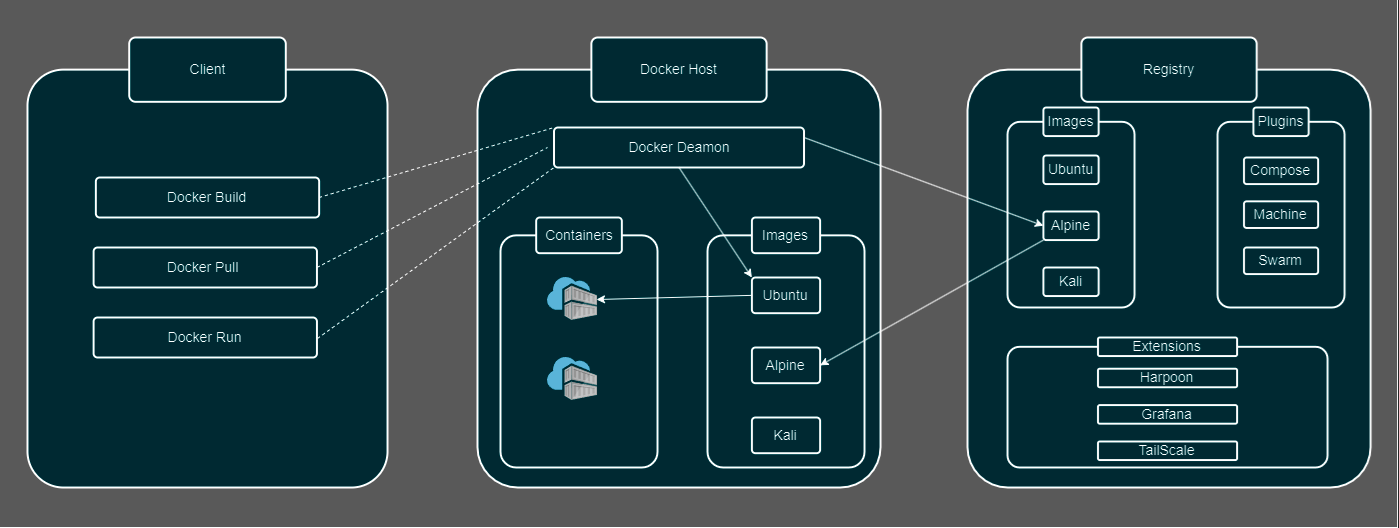
\includegraphics[width=1\textwidth]{Docker_Architecture.png}  % Sostituisci 'nome_immagine' con il nome del tuo file immagine e l'estensione
    \caption{Architettura Docker}
    \label{fig:DockerArchitecture}
\end{figure}

Di seguito una spiegazione di tutti gli elementi che intervengono nella creazione di un container:

\begin{itemize}
    \item \textbf{Docker Client}: Rappresenta la macchina fisica nel quale è installato Docker. Può comunicare con il controller principale (Docker Host) tramite delle Rest API.
    Le chiamate che il client può effettuare sono le seguenti:
        \begin{itemize}
            \item \textit{Docker Pull}: viene utilizzato per scaricare un'immagine da un Registro. Il demone controllerà se questa immagine è presente nel registro locale indicato, altrimenti andrà a cercare online
                la versione più recente dal registro predefinito di Docker Hub.
            \item \textit{Docker Build}: questo comando permette la creazione di un'immagine dato un file di configurazione definito dall utente (deve avere il nome di Dockerfile) e una cartella di riferimento.
            \item \textit{Docker Run}: questa chiamata fa creare al demone un container con l'immagine specificata da linea di comando ed avvia il container.
        \end{itemize}
    \item \textbf{Docker Deamon}: è il cuore dell'architettura di Docker. Il ruolo del docker deamon(anche chiamato dockerd) è di ascoltare le richieste tramite call API del client e gestire il registro Docker dove sono contenute
        le immagini, i plugin e le estensioni. Inoltre può comunicare con altri demoni per gestire i servizi Docker.
    \item \textbf{Docker Registry}: è  una zona di memoria che memorizza le immagini Docker. In questa zona sono anche presenti eventuali plugin installati su Docker e le estensioni sviluppate per sfruttare i servizi di Docker.
        Talvolta potrebbe capitare che le immagini ricercate nel registro non sono presenti, ed in questo caso viene effettuato un collegamento diretto con un registro pubblico online definito Docker Hub per poter usufruire di alcune
        immagini già pronte.
\end{itemize}


Ha senso inserire anche come si scrive un dockerfile con esempi di comando o no?

\section{Il tool Compose}

\subsection{Introduzione}
Come si è potuto notare nella sezione precedente, Docker garantisce un grado di flessibilità molto elevato che consente di creare sia container che svolgono ruoli molto semplici che container più articolati, i quali richiedono anche l'installazione di diverse
librerie tramite Dockerfile. Tuttavia capita molto spesso che isolare un container da  tutti gli altri sia una limitazione in quanto per svolgere determinati task due o più macchine virtuali devono potere comunicare efficacemente, inoltre la gestione
di reti complesse tramite singoli Dockerfile e linea di comando può risultare tediosa e molto scomoda da utilizzare. Basti pensare che nel caso di un container non funzionante bisognerebbe modificare non solo il Dockerfile del singolo elemento, ma anche rieseguire tutte le chiamate
di sistema per fare rebuild dell'ambiente virtuale. \\
Per venire incontro a questi problemi molto comuni nello sviluppo di applicazioni aziendali, Docker propone delle soluzioni innovative e che cercano non solo di proporre una soluzione ai problemi sopracitati , ma anche di introdurre dei meccanismi di semplificazione per la gestione di reti complesse.
Più precisamente le caratteristiche di docker compose possono essere riassunte, come specificato nella documentazione\cite{docker-compose}, dalle seguenti:

\begin{enumerate}
    \item \textbf{Ambienti isolati multipli}: Il plugin fornisce la possibilità di definire il nome del progetto per isolare i vari ambienti di sviluppo. Inoltre, fornisce la possibilità di richiamare il nome di un progetto per istanziare molteplici copie dello stesso ambiente, per evitare che le build interferiscano fra loro o 
        per evitare che diversi progetti che hanno gli stessi nomi per i servizi definiti vadano in contrasto.
    \item \textbf{Conservare i volumi di dati}: compose memorizza e ricorda i container esistiti precedentemente. In questo modo è possibile, ogni volta che si avvia l'ambiente virtuale, trovare i container utilizzati nelle precedenti iterazioni e copiare i dati dal vecchio container a quello nuovo. 
        È quindi garantito che si evitino perdite di dati importanti fra le varie iterazioni. 
    \item \textbf{Reboot Efficiente}: questa proprietà consente di poter fare un reboot completo dell'ambiente virtuale evitando di istanziare nuovamente i container che non sono stati modificati. Compose è infatti in grado di riconoscere i cambiamenti effettuati in ogni container e nella fase di reboot del sistema verranno distrutti e ricreati
        solo gli elementi modificati, evitando di sovraccaricare la macchina con del calcolo computazionale inutile.
    \item \textbf{Variabili e Flessibilità}: all'interno dei file di configurazione dell'ambiente virtuale è possibile definire variabili locali. Grazie ad esse è possibile creare delle configurazioni custom a seconda dell'utente o dell'ambiente fisico del sistema.
\end{enumerate}

Per poter definire un ambiente virtuale tramite un unico file di configurazione, docker-compose accetta come input un file YAML che definisce tutti gli elementi presenti da virtualizzare. 

\subsection{YAML}
YAML\cite{yaml}, acronimo di "Yet Another Markup Language", è un formato di serializzazione dei dati universamentalmente utilizzato grazie alla sua semplicità, facilità di scrittura e di lettuera e comprensione.
Queste caratteristiche sono ottenibili grazie a diversi elementi che questo formato ha derivato da linguaggi come Pearl, C o Python, fornendo sia allo sviluppatore che al lettore dei file una sintassi semplice e di immediata comprensione, come l'utilizzo dei caratteri di indentazione per definire i blocchi (allo stesso modo di Python) o la definizione
dei dati con mappe chiave valore come i file JSON.\\
Grazie a queste sue caratteristiche YAML è uno dei formati più utilizzati per la scrittura di file di configurazione, per scambiare dati fra programmi che utilizzano diversi linguaggi di programmazione o rappresentare dati molto complessi in modo chiaro e leggibile da un utente.
Per fornire maggiore contesto, si propone un esempio di definizione di un ipotetico file YAML:

\begin{lstlisting}[style=yaml,caption={Esempio definizione di un file YAML},label=lst:yamlexample]
    topology_name: "Example"
    vertices: 
        node1:
            name: "Alfa"
            ip: "120.10.0.1"

        node2:
            name: "Beta"
            ip: "120.10.0.2"
        node3:
            name: "Gamma"
            ip: "120.10.0.3"
    
    edges:
        edge1:
            name:"Alfa-Beta"
            ipstart: "120.10.0.1"
            ipend: "120.10.0.2"
        edge2:
            name:"Alfa-Gamma"
            ipstart: "120.10.0.1"
            ipend: "120.10.0.3"
        edge3:
            name:"Gamma-Beta"
            ipstart: "120.10.0.3"
            ipend: "120.10.0.2"   

\end{lstlisting}

Come si può notare, le somiglianze con un file JSON sono evidenti. In questo esempio vi è la definizione di un grafo, infatti è presente la definizione
degli archi e dei vertici. Il gruppo dei vertici è formato a sua volta da 3 sottogruppi, ciascuno rappresentante un nodo che è definito all'interno della 
topologia con nome ed ip. Analogamente, anche il gruppo degli archi contiene 3 sottoinsiemi, che definiscono i vari archi della topologia di rete dandogli un nome e definendo
l'ip di partenza e di destinazione di ogni arco.\\

\subsection{Services e Networking}
All'interno del plugin docker-compose è quindi possibile utilizzare un unico file YAML che definisce e stabilisce le relazioni fra tutti i container. Più precisamente all'interno
di un file è possibile definire, ad alto livello, i seguenti elementi:

\begin{itemize}
    \item \textbf{Services}: Come è possibile ricavare dalla documentazione\cite{composeservices}"Un servizio è una definizione astratta di una risorsa di elaborazione all'interno di un'applica-zione che può essere scalata o sostituita indipendentemente da altri componenti. 
    I servizi sono supportati da un insieme di contenitori, gestiti dalla piattaforma in base ai requisiti di replicazione e ai vincoli di posizionamento. Poiché i servizi sono supportati da contenitori, sono definiti da un'immagine Docker e un insieme di argomenti di runtime."
    Tramite la definizione di questi servizi è quindi possibile definire quali container il nostro sistema monterà e utilizzerà. Al fine di questo lavoro di tesi ogni container rappresenta un nodo all'interno della topologia di rete che verrà presa in esempio. La funzionalità del
    singolo nodo di rete verrà poi specificata all'interno dello stesso servizio. È infatti possibile definire, all'interno di ogni servizio, numerosi elementi che permettono di personalizzare il singolo servizio a preferenza dell'utente, i più importanti sono:\\

    \begin{itemize}
        \item \textit{Volumes}: rappresentano memorie persistenti istanziate al momento di avvio del container dall'host fisico. Questo permette quindi di poter istanziare dei container che contengono fin dall'inizio dei file di configurazione necessari. A differenza delle macchine virtuali, montare un volume
            non rappresenta una porzione di memoria condivisa fra il container e la macchina ospitante, in quanto questo negherebbe il requisito di isolamento del container, quanto piuttosto una modo per gestire i dati che devono essere conservati anche dopo che un container è stato arrestato o eliminato.
        \item \textit{Configs}: è un attributo possibile in fase di definizione del servizio, che consente di gestire le configurazioni distribuite, ovvero di fornire al servizio i file di configurazione necessari durante la fase di esecuzione del container.  
        \item \textit{Secrets}: questo attributo è molto simile ai configs definiti precedentemente, con la differenza principale di proteggere dati considerati sensibili o importanti, come delle password o delle chiavi private di crittazione. Un servizio può quindi accedere ai file solo se viene definito esplicitamente
            l'attributo "secret" su quel file.
    \end{itemize}

\item \textbf{Networks}: Le reti sono il secondo macro elemento definibile all'interno del file per docker-docker compose. All'interno è possibile definire i metodi di comunicazione fra i vari container, definendo delle reti all'interno delle quali i vari container possono comunicare. È importante sottolineare che 
    non è sufficiente definire all'interno di questo elemento una rete affinchè i container si connettano, ma è obbligatorio inserire all'interno di ogni servizio appartenente alla rete l'elemento "network" specificando il nome della rete che viene definita in questa sezione. Attraverso queste reti è possibile anche 
    configurare le interfacce di rete per i bridge, gli indirizzi ip per i client ed i server esplicitamente, favorendo così la comunicazione all'interno dell'ambiente virtuale e testando tramite i comandi da terminale noti come il ping. \\
    Analogamente ai servizi, anche le reti hanno a disposizione degli attributi che è possibile definire per personalizzare la rete:

    \begin{itemize}
        \item \textit{driver}: viene utilizzato per specificare il driver di rete da utilizzare. Al fine di questa tesi il driver principale utilizzato è il "bridge" che consente ai container di comunicare tra loro sullo stesso host tramite il bridge Docker predefinito.
        \item \textit{ipam}:  permette la gestione degli indirizzi ip per la rete in questione. Consente non solo di definire un indirizzo ip, ma anche di definire multiple interfacce di rete e intere sottoreti utilizzando la classica notazione con "\textbackslash".
        \item \textit{internal}: specifica se la rete può essere accessibile solo da altri container all'interno della stessa applicazione, oppure anche da container esterni.
        \item \textit{external}: specifica se il network è esterno al file docker-compose. In questo caso, il network deve essere creato al di fuori del file yaml utilizzato all'interno di docker-compose.
        \item \textit{name}: permette di definire il nome di una rete, che sarà l'identificativo per tutti i servizi che vorranno accedervi.
        \item \textit{attachable}: specifica se i container possono essere connessi a questa rete. Se non è specificato esplicatemente dall'utente il valore di default è "true".
        
    \end{itemize}
\end{itemize}

Le caratteristiche del file di configurazione appena definite garantiscono quindi una completa personalizzazione dei container, fornendo anche un ottimo metodo di automatizzazione dei container.
Di seguito è presentato un esempio, mantenendo la topologia descritta in [\ref{lst:yamlexample}], di alcuni degli attributi che verranno utilizzati all'interno di questo lavoro di tesi per definire gli ambienti virtuali delle topologie di rete che verranno studiate: 

\begin{lstlisting}[style=yaml,caption={Esempio file di configurazione docker-compose},label=yamldocker]
    services: 
        host1:
            container_name: host1
            hostname: host1
            image: nginx
            cap_add: NET_ADMIN
            command: sh -c "route del default"
            networks:
                clients:
                    ipv4_address: 120.10.0.1

        host2:
            container_name: host2
            hostname: host2
            image: nginx
            cap_add: NET_ADMIN
            command: sh -c "route del default"
            networks:
                clients:
                    ipv4_address: 120.10.0.2
               
        host3:
            container_name: host3
            hostname: host3
            image: nginx
            cap_add: NET_ADMIN
            command: sh -c "route del default"
            networks:
                clients:
                    ipv4_address: 120.10.0.3
    networks:
        clients:
            name: clients
            driver: bridge
            ipam:
                driver: default
                config:
                    subnet: 120.10.0.0/24
                    gateway: 120.10.0.200
\end{lstlisting}